% Copyright (C) 2022 Haoqing Xu
% School of Artificial Intelligence, Southeast University.
% --------------------------------------------------------------------------
%
% This work may be distributed and/or modified under the
% conditions of the LaTeX Project Public License, either
% version 1.3c of this license or (at your option) any later
% version. This version of this license is in
%    http://www.latex-project.org/lppl/lppl-1-3c.txt
% and the latest version of this license is in
%    http://www.latex-project.org/lppl.txt
% and version 1.3 or later is part of all distributions of
% LaTeX version 2005/12/01 or later.
%
% This work has the LPPL maintenance status `maintained'.
% The Current Maintainer of this work is Haoqing Xu.
%
% Home Page of the Project: https://github.com/SuikaXhq/seu-bachelor-thesis-2022
\documentclass{seuthesis-2022}

\title{}{(此栏可删除)}
\author{}
\studentnum{}
\department{}
\major{}
\supervisor{}
\period{}

% 如果使用了AI
\useAi % 如果没有使用AI,注释掉这一行即可
\useAIForText  %对应 文本生成及内容修改 复选框
\useAIForData  %对应 数据、图表分析、代码调试 复选框
\useAIForOther %对应 其他:请具体说明 复选框
\useAITools{DeepSeek-V3} % 工具,版本号
\useAIProcedure{示例:输入哪些关键词或主题,指导 AI 工具生成或修改了内容} % 使用过程
\useAIPages{第二章1.1(P5)} % 章节(页码)

% 如果没使用AI
\notUseAIStatement{填写示例:在本人毕业论文(设计)的撰写过程中,未使用任何生成式人工智能辅助工具。所有内容均由本人独立撰写和创作完成,能够确保学术诚信,不存在任何AI生成的内容。}

% AI情况说明表导师意见部分
\useAISupervisorAttitude{意见:}

\begin{document}

\maketitle
\makedeclaration
\makeai % 创建AI情况说明表

\frontmatter
\begin{abstract}[zh]
  摘要内容独立于正文而存在,是论文内容高度概括的简要陈述,应准确、具体、完整地概括论文的主要信息,内容包括研究目的、方法、过程、成果、结论及主要创新之处等,不含图表,不加注释,具有独立性和完整性,一般为400字左右。
  
  “摘要”用三号黑体加粗居中,“摘”与“要”之间空4个半角空格。摘要正文内容用小四号宋体,固定1.5倍行距。
  
  论文的关键词是反映毕业设计(论文)主题内容的名词,一般为3-5个,排在摘要正文部分下方。关键词与摘要之间空一行。关键词之间用逗号分开,最后一个关键词后不加标点符号。
  \keywords{关键词1,关键词2,关键词3,关键词4}
\end{abstract}

\begin{abstract}[en]
  英文摘要应与中文摘相对应,250个实词左右。采用第三人称介绍该学位论文内容,叙述的基本时态为一般现在时,确实需要强调过去的事情或者已经完成的行为才使用过去时、完成时等其他时态。
  
  ABSTRACT为三号Times New Roman加粗居中。
  
  英文摘要正文为小四号Times New Roman,固定1.5倍行距。英文关键词“KEY WORDS”大写,其后的关键词第一个字母大写,关键词之间用半角逗号隔开。
  \keywords{Keywords1,Keywords2,Keywords3,Keywords4}
\end{abstract}

\tableofcontents

\mainmatter
\chapter{绪论}
\section{课题背景和意义}
绪论部分主要论述选题的意义、国内外研究现状以及本文主要研究的内容、研究思路以及内容安排等。

章标题为三号黑体加粗居中;一级节标题(如,2.1 本文研究内容):四号黑体居左;二级节标题(如,2.1.1 实验方法):小四号宋体居左。

正文部分为小四号宋体,行间距1.5倍行距,首行缩进2个字符。

\section{研究现状}

\section{本文研究内容}

\chapter{正文}
正文部分每一章应另起页书写书写,层次要清楚,内容要有逻辑性,正文一般不少于15000字。正文部分因学科、选题特点可有差异,但必须言之成理,论据可靠,严格遵循本学科国际通行的学术规范。

中文为小四号宋体,英文及数字为小四号Times New Roman,首行缩进2个字符,行间距为1.5倍。

\section{插图格式要求}
插图力求精炼,且每个插图均应有图序和图名。图序与图名位于插图下方,图序一般按章节编排,如图1-1(第一章第1个图),在插图较少时可以全文连续编序,如图10。

如一个插图由两个及以上的分图组成,分图用(a)、(b)、(c)等标出,并标出分图名。

简单文字图可用WORD直接绘制,复杂的图考虑使用相应的图形绘制软件完成,以提高图形表达质量。

插图居中排列,与上文文本之间空一行。图序图名设置为五号宋体居中,图序与图名之间空一格。

引用:图 \ref{fig:1}、图 \ref{fig:2}、图 \ref{fig:2a}、图 \ref{fig:2b} 的引用示例(见tex文件)。

\begin{figure}[H]
    \centering
    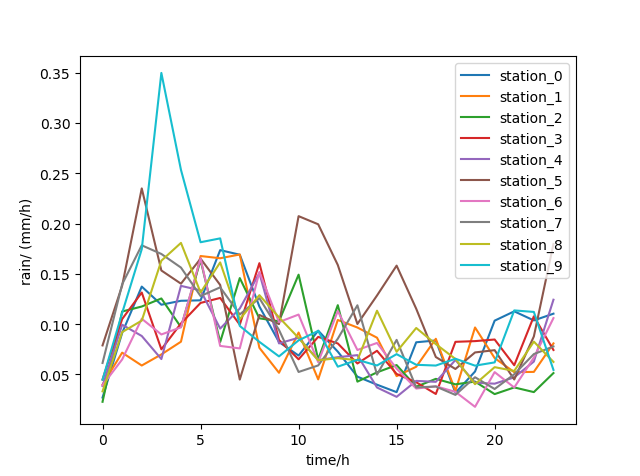
\includegraphics[width=0.5\linewidth]{fig/降水量均值分布图.png}
    \caption{每小时降水量24小时均值分布图}
    \label{fig:1}
\end{figure}

\begin{figure}[H]
    \centering
    \subcaptionbox{速度障碍集合\label{fig:2a}}
      {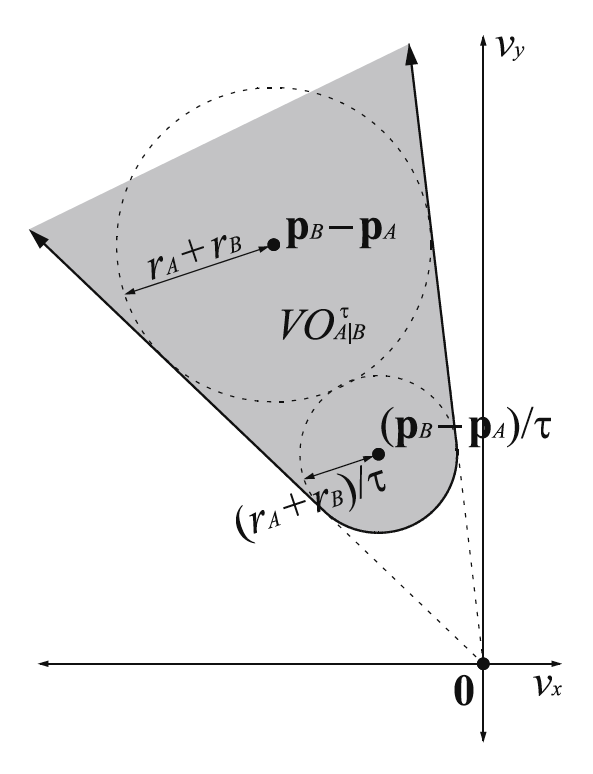
\includegraphics[width=0.3\linewidth]{fig/速度障碍集合.png}}
    \subcaptionbox{速度障碍集合\label{fig:2b}}
      {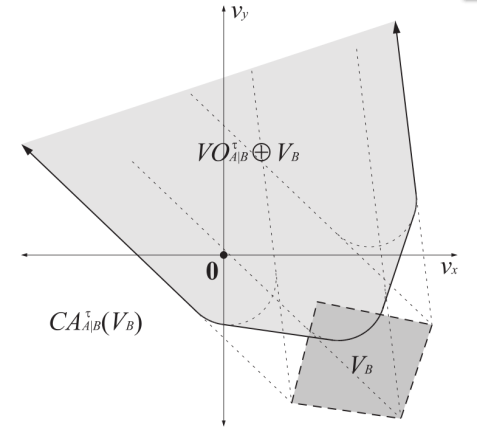
\includegraphics[width=0.4\linewidth]{fig/避免碰撞集合.png}}
    \caption{速度障碍法速度选择}
    \label{fig:2}
\end{figure}

\section{表格格式要求}
表格的结构应简洁,一律采用三线表,应有表序和表名,且表序和表名位于表格上方。表格可以逐章单独编序(如:表2.1),也可以统一编序(如:表10),采用哪种方式应和插图及公式的编序方式统一。表序必须连续,不得重复或跳跃。

表格无法在同一页排版时,可以用续表的形式另页书写,续表需在表格右上角表序前加“续”字,如“续表2.1”,并重复表头。

表格居中,边框为黑色直线1磅,中文为五号宋体,英文及数字为五号Times New Roman字体,表序与表名之间空一格,表格与下文之间空一行。需要注意必须在tabular环境前手动指定字号(见tex文件)。

引用:表 \ref{tab:1} 的引用示例(见tex文件)。

\begin{table}[H]
  \centering
  \caption{降水率分级统计}
  \label{tab:1}
  \small
  \begin{tabular}{ccc}
    \toprule
    降水率(mm/h)分级 & 该等级所占比例(\%) & 降水等级描述\\
    \midrule
    $0\le x< 0.5$ & 90.36 & 没有雨或雨很小\\
    $0.5\le x< 2.0$ & 6.41 & 小雨\\
    $2.0\le x< 5.0$ & 2.04 & 中雨\\
    $5.0\le x< 10.0$ & 0.10 & 大雨\\
    \bottomrule
  \end{tabular}
\end{table}

\section{表达式}
论文中的公式应注序号并加圆括号,序号一律用阿拉伯数字连续编序(如(28))或逐章编序(如(3.6)),编号方式应与插图、表格方式一致。序号排在版面右侧,且距右边距离相等。公式与序号之间不加虚线。

长公式在一行无法写完的情况下,原则上应在等号(或数学符号,如“+”、“-”号)处换行,数学符号在换行的行首。

公式及文字中的一般变量(或一般函数)(如坐标X、Y,电压V,频率f)宜用斜体,矢量用粗斜体如S或白斜体上加单箭头,常用函数(如三角函数cos、对数函数ln等)、数字运算符、化学元素符号及分子式、单位符号、产品代号、人名地名的外文字母等用正体。

公式排版时可选中模板中的“公式式样”,先将光标移至公式前,按“Tab”键,公式居中;再将光标移至编号前,按“Tab”键移动一个制表符位置,使公式编号右对齐。
\begin{equation}\label{eq:1}
  V_{cell}=E_{OCV}-V_{oct}-V_{ohm}-V_{conc}
  \end{equation}
引用:公式 \eqref{eq:1} 的引用示例(见tex文件)。

  
\section{注释}
正文中有个别名词或情况需要解释时,可加注说明,注释采用页末注(将注文放在加注页的下端)。在引文的右上角标注序号\circled{1}、\circled{2}、……,如“马尔可夫链\footnote{马尔科夫链表示}”。若在同一页中有两个以上的注时,按各注出现的先后,顺序编号。引文序号,以页为单位,且注释只限于写在注释符号出现的同页,不得隔页。

注释采用小五号宋体,英文及数字为小五号Times New Roman字体,利用“引用”插入脚注功能插入。

\chapter{总结与展望}
\section{工作总结}
最后一章结论与展望着重总结论文的创新点或新见解及研究展望或建议。

结论是对论文主要研究结果、论点的提炼与概括,应准确、简明、完整、有条理,使人看后就能全面了解论文的意义、目的和工作内容。主要阐述自己的创造性工作及所取得的研究成果在本学术领域中的地位、作用和意义。

结论要严格区分自己取得的成果与导师及他人的科研工作成果。在评价自己的研究工作成果时,要实事求是,除非有足够的证据表明自己的研究是“首次”的、“领先”的、“填补空白”的,否则应避免使用这些或类似词语。

\section{工作展望}
展望或建议,是在总结研究工作和现有结论的基础上,对该领域今后的发展方向及重要研究内容进行预测,同时对所获研究结果的应用前景和社会影响加以评价,从而对今后的研究有所启发。

\nocite{*}
\bibliographystyle{gbt7714-numerical}
\bibliography{reference.bib}

\appendix
\chapter{附录名称}
对于一些不宜放入正文中、但作为毕业设计(论文)又不可残缺的组成部分或具有重要参考价值的内容,可编入毕业设计(论文)的附录中,例如,正文内过于冗长的公式推导、方便他人阅读所需的辅助性数学工具或表格、重复性数据和图表、非常必要的程序说明和程序全文、关键调查问卷或方案等。

附录的格式与正文相同,如有多个附录需依顺序用大写字母A,B,C,……编序号,如附录A,附录B,附录C,……。只有一个附录时也要编序号,即附录A。每个附录应有标题,如:“附录A 参考文献著录规则及注意事项”。

附录一般与论文全文装订在一起,与正文一起编页码。


\begin{acknowledgement}
学位论文正文和附录之后,一般应放置致谢(后记或说明),主要感谢指导老师和对论文工作有直接贡献和帮助的人士和单位。致谢言语应谦虚诚恳,实事求是。字数一般不超过1000个汉字。

“致谢”用三号黑体加粗居中,两字之间空4个半角空格。致谢内容为小四号宋体,1.5倍行距。
\end{acknowledgement}
\end{document}